\documentclass{article}

% Language setting
% Replace `english' with e.g. `spanish' to change the document language
\usepackage[english]{babel}
\usepackage{graphicx}
% Set page size and margins
% Replace `letterpaper' with`a4paper' for UK/EU standard size
\usepackage[letterpaper,top=2cm,bottom=2cm,left=3cm,right=3cm,marginparwidth=1.75cm]{geometry}

% Useful packages
\usepackage{amsmath,amsthm,amssymb}
\usepackage{enumitem}




\title{Problem Set 6}
\author{Leah Pomerantz}

\begin{document}
\maketitle


\section{Problem 3 - Data Cleaning}

I used some of the data from the NLSY79 cohort. I started with several variables describing the 79 cohort and filtered down to just the variables I was interested in making graphs of, keeping the ID number, Sample ID number, Race, Sex, AFQT score, and the Highest-grade-ever-completed variable. To make the data more legible and easier to work with, I changed the default names of the variables to the following: "CaseID", "SampleID", "Race", "Sex", "AFTQ", and "HGC\_Ever". Once I had just the variables I was interested in, I filtered out all the NA's in the data. I checked the number of observations before and after and found that I only lost around 300 observations. Since I still had over 11,000, I wasn't terribly worried and decided that this would suffice.

\section{Problem 5 - Images}


\begin{figure}[htp]
    \centering
    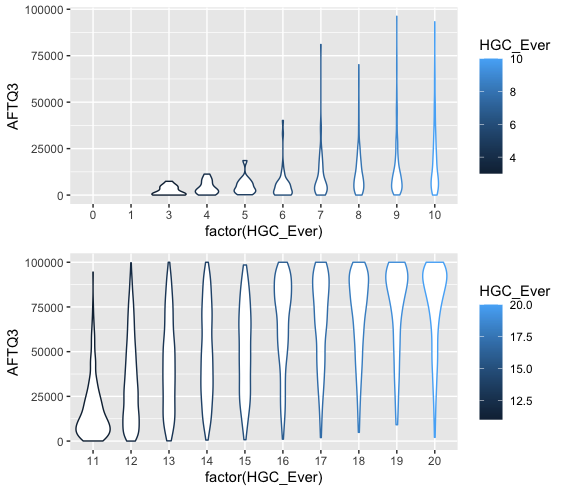
\includegraphics[width=8cm]{Images/PS6a_Pomerantz.png}
    \caption{Intelligence Scores vs. Education}
    \label{fig:comp}
\end{figure}

The above figure is a violin plot with education levels on the x-axis and intelligence scores on the y-axis. The nice thing about violin plots is that we get a look at a combination of a mirrored density plot and a boxplot. So we can see density and we can see tips and tails. This shows us a visual of what we would expect: when education levels are lower, the intelligence scores are lower. We also see a big change in shape from 11 to 12, which shows the line in years completed between high school dropouts (after junior year) and people who completed high school. We see another change from 15 to 16 years, representing a college drop-out (junior year) and someone who completed college. This difference becomes more and more pronounced as we move along in years of post-college education. The biggest takeaway is that the density and distribution of intelligence scores changes with years of education, and that the difference between completing these levels of education vs. not is visible on the graph. This doesn't necessarily represent actual intelligence; we cannot infer anything about causality from the graph. However, we can visualize an observation that could be a jumping-off point for a regression analysis.

\begin{figure}[htp]
    \centering
    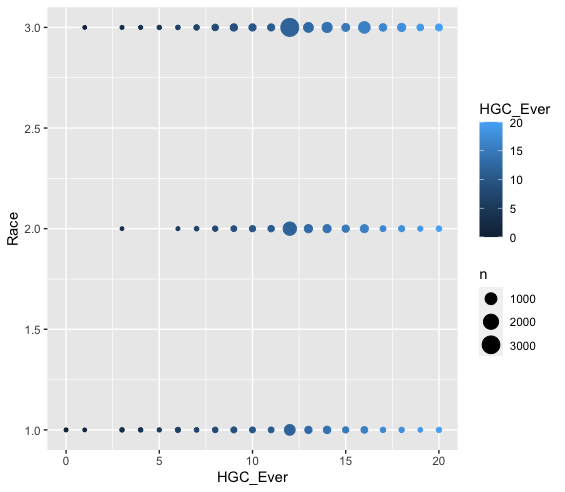
\includegraphics[width=8cm]{Images/PS6b_Pomerantz.png}
    \caption{Race vs. Education}
    \label{fig:comp1}
\end{figure}

This figure shows us a distribution of Race vs. years of education, with the size of the dots representing number of observations. It again shows us a helpful visualization. With how the data are coded, 1 is Black, 2 is Hispanic, and 3 is non-Black/non-Hispanic. We can see that the education level for Black persons has a higher variance than the other racial categories. We also see that the non-Black/non-Hispanic has a higher density at higher education levels. Graphs are also helpful for seeing holes in our data, and we can see some here. It would be much more useful to have more categories for race to see which group is driving the higher level of measured education levels. It also might be helpful to split this into three different graphs based on race, create vertical dotplots measuring count for each education level, one for each group, and then look at the graphs side-by-side. It looks like this type of graph might be an oversimplification for this category. Nevertheless, the graph gives us helpful information!

\begin{figure}[htp]
    \centering
    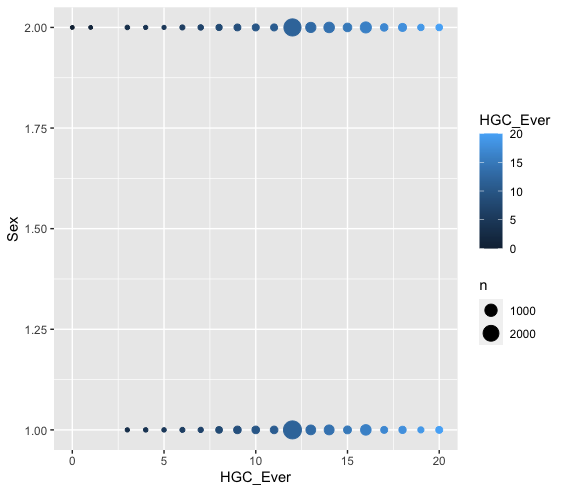
\includegraphics[width=8cm]{Images/PS6c_Pomerantz.png}
    \caption{Sex vs. Education}
    \label{fig:comp2}
\end{figure}

This figure again shows us an unsurprising result. The data are encoded such that 1 means male and 2 means female. As is fitting for their age group, men have their median at a higher level than women and they have a lower variance. After high school, the difference no longer appears to be big. It looks like more women are high school dropouts than men, but, given high school completion, more women go to college than men. This is a slightly surprising result.

\end{document}